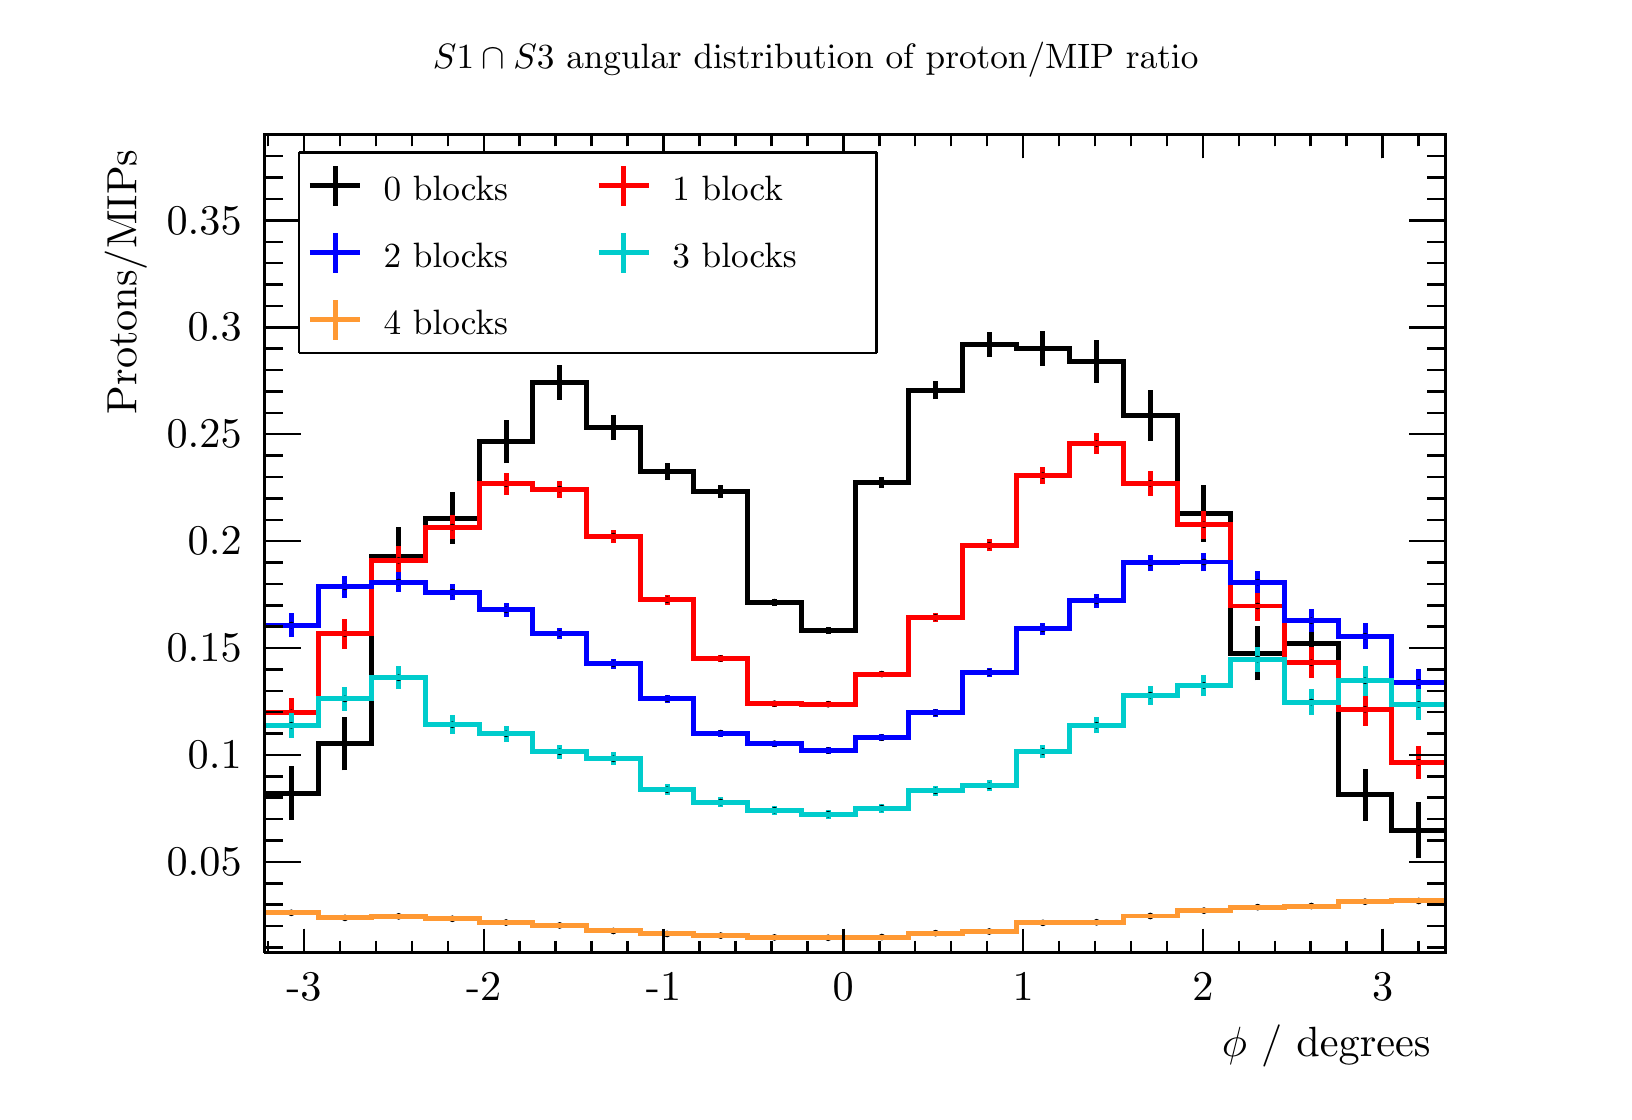
\begin{tikzpicture}
\pgfdeclareplotmark{cross} {
\pgfpathmoveto{\pgfpoint{-0.3\pgfplotmarksize}{\pgfplotmarksize}}
\pgfpathlineto{\pgfpoint{+0.3\pgfplotmarksize}{\pgfplotmarksize}}
\pgfpathlineto{\pgfpoint{+0.3\pgfplotmarksize}{0.3\pgfplotmarksize}}
\pgfpathlineto{\pgfpoint{+1\pgfplotmarksize}{0.3\pgfplotmarksize}}
\pgfpathlineto{\pgfpoint{+1\pgfplotmarksize}{-0.3\pgfplotmarksize}}
\pgfpathlineto{\pgfpoint{+0.3\pgfplotmarksize}{-0.3\pgfplotmarksize}}
\pgfpathlineto{\pgfpoint{+0.3\pgfplotmarksize}{-1.\pgfplotmarksize}}
\pgfpathlineto{\pgfpoint{-0.3\pgfplotmarksize}{-1.\pgfplotmarksize}}
\pgfpathlineto{\pgfpoint{-0.3\pgfplotmarksize}{-0.3\pgfplotmarksize}}
\pgfpathlineto{\pgfpoint{-1.\pgfplotmarksize}{-0.3\pgfplotmarksize}}
\pgfpathlineto{\pgfpoint{-1.\pgfplotmarksize}{0.3\pgfplotmarksize}}
\pgfpathlineto{\pgfpoint{-0.3\pgfplotmarksize}{0.3\pgfplotmarksize}}
\pgfpathclose
\pgfusepathqstroke
}
\pgfdeclareplotmark{cross*} {
\pgfpathmoveto{\pgfpoint{-0.3\pgfplotmarksize}{\pgfplotmarksize}}
\pgfpathlineto{\pgfpoint{+0.3\pgfplotmarksize}{\pgfplotmarksize}}
\pgfpathlineto{\pgfpoint{+0.3\pgfplotmarksize}{0.3\pgfplotmarksize}}
\pgfpathlineto{\pgfpoint{+1\pgfplotmarksize}{0.3\pgfplotmarksize}}
\pgfpathlineto{\pgfpoint{+1\pgfplotmarksize}{-0.3\pgfplotmarksize}}
\pgfpathlineto{\pgfpoint{+0.3\pgfplotmarksize}{-0.3\pgfplotmarksize}}
\pgfpathlineto{\pgfpoint{+0.3\pgfplotmarksize}{-1.\pgfplotmarksize}}
\pgfpathlineto{\pgfpoint{-0.3\pgfplotmarksize}{-1.\pgfplotmarksize}}
\pgfpathlineto{\pgfpoint{-0.3\pgfplotmarksize}{-0.3\pgfplotmarksize}}
\pgfpathlineto{\pgfpoint{-1.\pgfplotmarksize}{-0.3\pgfplotmarksize}}
\pgfpathlineto{\pgfpoint{-1.\pgfplotmarksize}{0.3\pgfplotmarksize}}
\pgfpathlineto{\pgfpoint{-0.3\pgfplotmarksize}{0.3\pgfplotmarksize}}
\pgfpathclose
\pgfusepathqfillstroke
}
\pgfdeclareplotmark{newstar} {
\pgfpathmoveto{\pgfqpoint{0pt}{\pgfplotmarksize}}
\pgfpathlineto{\pgfqpointpolar{44}{0.5\pgfplotmarksize}}
\pgfpathlineto{\pgfqpointpolar{18}{\pgfplotmarksize}}
\pgfpathlineto{\pgfqpointpolar{-20}{0.5\pgfplotmarksize}}
\pgfpathlineto{\pgfqpointpolar{-54}{\pgfplotmarksize}}
\pgfpathlineto{\pgfqpointpolar{-90}{0.5\pgfplotmarksize}}
\pgfpathlineto{\pgfqpointpolar{234}{\pgfplotmarksize}}
\pgfpathlineto{\pgfqpointpolar{198}{0.5\pgfplotmarksize}}
\pgfpathlineto{\pgfqpointpolar{162}{\pgfplotmarksize}}
\pgfpathlineto{\pgfqpointpolar{134}{0.5\pgfplotmarksize}}
\pgfpathclose
\pgfusepathqstroke
}
\pgfdeclareplotmark{newstar*} {
\pgfpathmoveto{\pgfqpoint{0pt}{\pgfplotmarksize}}
\pgfpathlineto{\pgfqpointpolar{44}{0.5\pgfplotmarksize}}
\pgfpathlineto{\pgfqpointpolar{18}{\pgfplotmarksize}}
\pgfpathlineto{\pgfqpointpolar{-20}{0.5\pgfplotmarksize}}
\pgfpathlineto{\pgfqpointpolar{-54}{\pgfplotmarksize}}
\pgfpathlineto{\pgfqpointpolar{-90}{0.5\pgfplotmarksize}}
\pgfpathlineto{\pgfqpointpolar{234}{\pgfplotmarksize}}
\pgfpathlineto{\pgfqpointpolar{198}{0.5\pgfplotmarksize}}
\pgfpathlineto{\pgfqpointpolar{162}{\pgfplotmarksize}}
\pgfpathlineto{\pgfqpointpolar{134}{0.5\pgfplotmarksize}}
\pgfpathclose
\pgfusepathqfillstroke
}
\definecolor{c}{rgb}{1,1,1};
\draw [color=c, fill=c] (0,0) rectangle (20,13.4957);
\draw [color=c, fill=c] (3,1.75444) rectangle (18,12.1461);
\definecolor{c}{rgb}{0,0,0};
\draw [c,line width=0.9] (3,1.75444) -- (3,12.1461) -- (18,12.1461) -- (18,1.75444) -- (3,1.75444);
\definecolor{c}{rgb}{1,1,1};
\draw [color=c, fill=c] (3,1.75444) rectangle (18,12.1461);
\definecolor{c}{rgb}{0,0,0};
\draw [c,line width=0.9] (3,1.75444) -- (3,12.1461) -- (18,12.1461) -- (18,1.75444) -- (3,1.75444);
\draw [c,line width=0.9] (3,1.75444) -- (3.68182,1.75444) -- (3.68182,1.75444) -- (4.36364,1.75444) -- (4.36364,1.75444) -- (5.04545,1.75444) -- (5.04545,1.75444) -- (5.72727,1.75444) -- (5.72727,1.75444) -- (6.40909,1.75444) -- (6.40909,1.75444) --
 (7.09091,1.75444) -- (7.09091,1.75444) -- (7.77273,1.75444) -- (7.77273,1.75444) -- (8.45455,1.75444) -- (8.45455,1.75444) -- (9.13636,1.75444) -- (9.13636,1.75444) -- (9.81818,1.75444) -- (9.81818,1.75444) -- (10.5,1.75444) -- (10.5,1.75444) --
 (11.1818,1.75444) -- (11.1818,1.75444) -- (11.8636,1.75444) -- (11.8636,1.75444) -- (12.5455,1.75444) -- (12.5455,1.75444) -- (13.2273,1.75444) -- (13.2273,1.75444) -- (13.9091,1.75444) -- (13.9091,1.75444) -- (14.5909,1.75444) -- (14.5909,1.75444)
 -- (15.2727,1.75444) -- (15.2727,1.75444) -- (15.9545,1.75444) -- (15.9545,1.75444) -- (16.6364,1.75444) -- (16.6364,1.75444) -- (17.3182,1.75444) -- (17.3182,1.75444) -- (18,1.75444);
\draw [c,line width=0.9] (3,1.75444) -- (18,1.75444);
\draw [c,line width=0.9] (3.50228,2.05809) -- (3.50228,1.75444);
\draw [c,line width=0.9] (3.9589,1.90627) -- (3.9589,1.75444);
\draw [c,line width=0.9] (4.41553,1.90627) -- (4.41553,1.75444);
\draw [c,line width=0.9] (4.87215,1.90627) -- (4.87215,1.75444);
\draw [c,line width=0.9] (5.32877,1.90627) -- (5.32877,1.75444);
\draw [c,line width=0.9] (5.78539,2.05809) -- (5.78539,1.75444);
\draw [c,line width=0.9] (6.24201,1.90627) -- (6.24201,1.75444);
\draw [c,line width=0.9] (6.69863,1.90627) -- (6.69863,1.75444);
\draw [c,line width=0.9] (7.15525,1.90627) -- (7.15525,1.75444);
\draw [c,line width=0.9] (7.61187,1.90627) -- (7.61187,1.75444);
\draw [c,line width=0.9] (8.06849,2.05809) -- (8.06849,1.75444);
\draw [c,line width=0.9] (8.52511,1.90627) -- (8.52511,1.75444);
\draw [c,line width=0.9] (8.98174,1.90627) -- (8.98174,1.75444);
\draw [c,line width=0.9] (9.43836,1.90627) -- (9.43836,1.75444);
\draw [c,line width=0.9] (9.89498,1.90627) -- (9.89498,1.75444);
\draw [c,line width=0.9] (10.3516,2.05809) -- (10.3516,1.75444);
\draw [c,line width=0.9] (10.8082,1.90627) -- (10.8082,1.75444);
\draw [c,line width=0.9] (11.2648,1.90627) -- (11.2648,1.75444);
\draw [c,line width=0.9] (11.7215,1.90627) -- (11.7215,1.75444);
\draw [c,line width=0.9] (12.1781,1.90627) -- (12.1781,1.75444);
\draw [c,line width=0.9] (12.6347,2.05809) -- (12.6347,1.75444);
\draw [c,line width=0.9] (13.0913,1.90627) -- (13.0913,1.75444);
\draw [c,line width=0.9] (13.5479,1.90627) -- (13.5479,1.75444);
\draw [c,line width=0.9] (14.0046,1.90627) -- (14.0046,1.75444);
\draw [c,line width=0.9] (14.4612,1.90627) -- (14.4612,1.75444);
\draw [c,line width=0.9] (14.9178,2.05809) -- (14.9178,1.75444);
\draw [c,line width=0.9] (15.3744,1.90627) -- (15.3744,1.75444);
\draw [c,line width=0.9] (15.831,1.90627) -- (15.831,1.75444);
\draw [c,line width=0.9] (16.2877,1.90627) -- (16.2877,1.75444);
\draw [c,line width=0.9] (16.7443,1.90627) -- (16.7443,1.75444);
\draw [c,line width=0.9] (17.2009,2.05809) -- (17.2009,1.75444);
\draw [c,line width=0.9] (3.50228,2.05809) -- (3.50228,1.75444);
\draw [c,line width=0.9] (3.04566,1.90627) -- (3.04566,1.75444);
\draw [c,line width=0.9] (17.2009,2.05809) -- (17.2009,1.75444);
\draw [c,line width=0.9] (17.6575,1.90627) -- (17.6575,1.75444);
\draw [anchor=base] (3.50228,1.14713) node[scale=1.52731, color=c, rotate=0]{-3};
\draw [anchor=base] (5.78539,1.14713) node[scale=1.52731, color=c, rotate=0]{-2};
\draw [anchor=base] (8.06849,1.14713) node[scale=1.52731, color=c, rotate=0]{-1};
\draw [anchor=base] (10.3516,1.14713) node[scale=1.52731, color=c, rotate=0]{0};
\draw [anchor=base] (12.6347,1.14713) node[scale=1.52731, color=c, rotate=0]{1};
\draw [anchor=base] (14.9178,1.14713) node[scale=1.52731, color=c, rotate=0]{2};
\draw [anchor=base] (17.2009,1.14713) node[scale=1.52731, color=c, rotate=0]{3};
\draw [anchor= east] (18,0.566819) node[scale=1.52731, color=c, rotate=0]{$\phi$ / degrees};
\draw [c,line width=0.9] (3,12.1461) -- (18,12.1461);
\draw [c,line width=0.9] (3.50228,11.8425) -- (3.50228,12.1461);
\draw [c,line width=0.9] (3.9589,11.9943) -- (3.9589,12.1461);
\draw [c,line width=0.9] (4.41553,11.9943) -- (4.41553,12.1461);
\draw [c,line width=0.9] (4.87215,11.9943) -- (4.87215,12.1461);
\draw [c,line width=0.9] (5.32877,11.9943) -- (5.32877,12.1461);
\draw [c,line width=0.9] (5.78539,11.8425) -- (5.78539,12.1461);
\draw [c,line width=0.9] (6.24201,11.9943) -- (6.24201,12.1461);
\draw [c,line width=0.9] (6.69863,11.9943) -- (6.69863,12.1461);
\draw [c,line width=0.9] (7.15525,11.9943) -- (7.15525,12.1461);
\draw [c,line width=0.9] (7.61187,11.9943) -- (7.61187,12.1461);
\draw [c,line width=0.9] (8.06849,11.8425) -- (8.06849,12.1461);
\draw [c,line width=0.9] (8.52511,11.9943) -- (8.52511,12.1461);
\draw [c,line width=0.9] (8.98174,11.9943) -- (8.98174,12.1461);
\draw [c,line width=0.9] (9.43836,11.9943) -- (9.43836,12.1461);
\draw [c,line width=0.9] (9.89498,11.9943) -- (9.89498,12.1461);
\draw [c,line width=0.9] (10.3516,11.8425) -- (10.3516,12.1461);
\draw [c,line width=0.9] (10.8082,11.9943) -- (10.8082,12.1461);
\draw [c,line width=0.9] (11.2648,11.9943) -- (11.2648,12.1461);
\draw [c,line width=0.9] (11.7215,11.9943) -- (11.7215,12.1461);
\draw [c,line width=0.9] (12.1781,11.9943) -- (12.1781,12.1461);
\draw [c,line width=0.9] (12.6347,11.8425) -- (12.6347,12.1461);
\draw [c,line width=0.9] (13.0913,11.9943) -- (13.0913,12.1461);
\draw [c,line width=0.9] (13.5479,11.9943) -- (13.5479,12.1461);
\draw [c,line width=0.9] (14.0046,11.9943) -- (14.0046,12.1461);
\draw [c,line width=0.9] (14.4612,11.9943) -- (14.4612,12.1461);
\draw [c,line width=0.9] (14.9178,11.8425) -- (14.9178,12.1461);
\draw [c,line width=0.9] (15.3744,11.9943) -- (15.3744,12.1461);
\draw [c,line width=0.9] (15.831,11.9943) -- (15.831,12.1461);
\draw [c,line width=0.9] (16.2877,11.9943) -- (16.2877,12.1461);
\draw [c,line width=0.9] (16.7443,11.9943) -- (16.7443,12.1461);
\draw [c,line width=0.9] (17.2009,11.8425) -- (17.2009,12.1461);
\draw [c,line width=0.9] (3.50228,11.8425) -- (3.50228,12.1461);
\draw [c,line width=0.9] (3.04566,11.9943) -- (3.04566,12.1461);
\draw [c,line width=0.9] (17.2009,11.8425) -- (17.2009,12.1461);
\draw [c,line width=0.9] (17.6575,11.9943) -- (17.6575,12.1461);
\draw [c,line width=0.9] (3,1.75444) -- (3,12.1461);
\draw [c,line width=0.9] (3.462,2.90832) -- (3,2.90832);
\draw [c,line width=0.9] (3.231,3.17988) -- (3,3.17988);
\draw [c,line width=0.9] (3.231,3.45144) -- (3,3.45144);
\draw [c,line width=0.9] (3.231,3.72299) -- (3,3.72299);
\draw [c,line width=0.9] (3.231,3.99455) -- (3,3.99455);
\draw [c,line width=0.9] (3.462,4.26611) -- (3,4.26611);
\draw [c,line width=0.9] (3.231,4.53766) -- (3,4.53766);
\draw [c,line width=0.9] (3.231,4.80922) -- (3,4.80922);
\draw [c,line width=0.9] (3.231,5.08077) -- (3,5.08077);
\draw [c,line width=0.9] (3.231,5.35233) -- (3,5.35233);
\draw [c,line width=0.9] (3.462,5.62389) -- (3,5.62389);
\draw [c,line width=0.9] (3.231,5.89544) -- (3,5.89544);
\draw [c,line width=0.9] (3.231,6.167) -- (3,6.167);
\draw [c,line width=0.9] (3.231,6.43856) -- (3,6.43856);
\draw [c,line width=0.9] (3.231,6.71011) -- (3,6.71011);
\draw [c,line width=0.9] (3.462,6.98167) -- (3,6.98167);
\draw [c,line width=0.9] (3.231,7.25322) -- (3,7.25322);
\draw [c,line width=0.9] (3.231,7.52478) -- (3,7.52478);
\draw [c,line width=0.9] (3.231,7.79634) -- (3,7.79634);
\draw [c,line width=0.9] (3.231,8.06789) -- (3,8.06789);
\draw [c,line width=0.9] (3.462,8.33945) -- (3,8.33945);
\draw [c,line width=0.9] (3.231,8.61101) -- (3,8.61101);
\draw [c,line width=0.9] (3.231,8.88256) -- (3,8.88256);
\draw [c,line width=0.9] (3.231,9.15412) -- (3,9.15412);
\draw [c,line width=0.9] (3.231,9.42568) -- (3,9.42568);
\draw [c,line width=0.9] (3.462,9.69723) -- (3,9.69723);
\draw [c,line width=0.9] (3.231,9.96879) -- (3,9.96879);
\draw [c,line width=0.9] (3.231,10.2403) -- (3,10.2403);
\draw [c,line width=0.9] (3.231,10.5119) -- (3,10.5119);
\draw [c,line width=0.9] (3.231,10.7835) -- (3,10.7835);
\draw [c,line width=0.9] (3.462,11.055) -- (3,11.055);
\draw [c,line width=0.9] (3.462,2.90832) -- (3,2.90832);
\draw [c,line width=0.9] (3.231,2.63677) -- (3,2.63677);
\draw [c,line width=0.9] (3.231,2.36521) -- (3,2.36521);
\draw [c,line width=0.9] (3.231,2.09365) -- (3,2.09365);
\draw [c,line width=0.9] (3.231,1.8221) -- (3,1.8221);
\draw [c,line width=0.9] (3.462,11.055) -- (3,11.055);
\draw [c,line width=0.9] (3.231,11.3266) -- (3,11.3266);
\draw [c,line width=0.9] (3.231,11.5981) -- (3,11.5981);
\draw [c,line width=0.9] (3.231,11.8697) -- (3,11.8697);
\draw [c,line width=0.9] (3.231,12.1412) -- (3,12.1412);
\draw [anchor= east] (2.9,2.90832) node[scale=1.52731, color=c, rotate=0]{0.05};
\draw [anchor= east] (2.9,4.26611) node[scale=1.52731, color=c, rotate=0]{0.1};
\draw [anchor= east] (2.9,5.62389) node[scale=1.52731, color=c, rotate=0]{0.15};
\draw [anchor= east] (2.9,6.98167) node[scale=1.52731, color=c, rotate=0]{0.2};
\draw [anchor= east] (2.9,8.33945) node[scale=1.52731, color=c, rotate=0]{0.25};
\draw [anchor= east] (2.9,9.69723) node[scale=1.52731, color=c, rotate=0]{0.3};
\draw [anchor= east] (2.9,11.055) node[scale=1.52731, color=c, rotate=0]{0.35};
\draw [anchor= east] (1.24,12.1461) node[scale=1.52731, color=c, rotate=90]{  Protons/MIPs};
\draw [c,line width=0.9] (18,1.75444) -- (18,12.1461);
\draw [c,line width=0.9] (17.538,2.90832) -- (18,2.90832);
\draw [c,line width=0.9] (17.769,3.17988) -- (18,3.17988);
\draw [c,line width=0.9] (17.769,3.45144) -- (18,3.45144);
\draw [c,line width=0.9] (17.769,3.72299) -- (18,3.72299);
\draw [c,line width=0.9] (17.769,3.99455) -- (18,3.99455);
\draw [c,line width=0.9] (17.538,4.26611) -- (18,4.26611);
\draw [c,line width=0.9] (17.769,4.53766) -- (18,4.53766);
\draw [c,line width=0.9] (17.769,4.80922) -- (18,4.80922);
\draw [c,line width=0.9] (17.769,5.08077) -- (18,5.08077);
\draw [c,line width=0.9] (17.769,5.35233) -- (18,5.35233);
\draw [c,line width=0.9] (17.538,5.62389) -- (18,5.62389);
\draw [c,line width=0.9] (17.769,5.89544) -- (18,5.89544);
\draw [c,line width=0.9] (17.769,6.167) -- (18,6.167);
\draw [c,line width=0.9] (17.769,6.43856) -- (18,6.43856);
\draw [c,line width=0.9] (17.769,6.71011) -- (18,6.71011);
\draw [c,line width=0.9] (17.538,6.98167) -- (18,6.98167);
\draw [c,line width=0.9] (17.769,7.25322) -- (18,7.25322);
\draw [c,line width=0.9] (17.769,7.52478) -- (18,7.52478);
\draw [c,line width=0.9] (17.769,7.79634) -- (18,7.79634);
\draw [c,line width=0.9] (17.769,8.06789) -- (18,8.06789);
\draw [c,line width=0.9] (17.538,8.33945) -- (18,8.33945);
\draw [c,line width=0.9] (17.769,8.61101) -- (18,8.61101);
\draw [c,line width=0.9] (17.769,8.88256) -- (18,8.88256);
\draw [c,line width=0.9] (17.769,9.15412) -- (18,9.15412);
\draw [c,line width=0.9] (17.769,9.42568) -- (18,9.42568);
\draw [c,line width=0.9] (17.538,9.69723) -- (18,9.69723);
\draw [c,line width=0.9] (17.769,9.96879) -- (18,9.96879);
\draw [c,line width=0.9] (17.769,10.2403) -- (18,10.2403);
\draw [c,line width=0.9] (17.769,10.5119) -- (18,10.5119);
\draw [c,line width=0.9] (17.769,10.7835) -- (18,10.7835);
\draw [c,line width=0.9] (17.538,11.055) -- (18,11.055);
\draw [c,line width=0.9] (17.538,2.90832) -- (18,2.90832);
\draw [c,line width=0.9] (17.769,2.63677) -- (18,2.63677);
\draw [c,line width=0.9] (17.769,2.36521) -- (18,2.36521);
\draw [c,line width=0.9] (17.769,2.09365) -- (18,2.09365);
\draw [c,line width=0.9] (17.769,1.8221) -- (18,1.8221);
\draw [c,line width=0.9] (17.538,11.055) -- (18,11.055);
\draw [c,line width=0.9] (17.769,11.3266) -- (18,11.3266);
\draw [c,line width=0.9] (17.769,11.5981) -- (18,11.5981);
\draw [c,line width=0.9] (17.769,11.8697) -- (18,11.8697);
\draw [c,line width=0.9] (17.769,12.1412) -- (18,12.1412);
\draw [c,line width=1.8] (3.34091,3.4416) -- (3.34091,3.78135);
\draw [c,line width=1.8] (3.34091,3.78135) -- (3.34091,4.1211);
\foreach \P in {(3.34091,3.78135)}{\draw[mark options={color=c,fill=c},mark size=2.402402pt,mark=*,mark size=1pt] plot coordinates {\P};}
\draw [c,line width=1.8] (4.02273,4.07152) -- (4.02273,4.4091);
\draw [c,line width=1.8] (4.02273,4.4091) -- (4.02273,4.74668);
\foreach \P in {(4.02273,4.4091)}{\draw[mark options={color=c,fill=c},mark size=2.402402pt,mark=*,mark size=1pt] plot coordinates {\P};}
\draw [c,line width=1.8] (4.70455,6.40225) -- (4.70455,6.78243);
\draw [c,line width=1.8] (4.70455,6.78243) -- (4.70455,7.16261);
\foreach \P in {(4.70455,6.78243)}{\draw[mark options={color=c,fill=c},mark size=2.402402pt,mark=*,mark size=1pt] plot coordinates {\P};}
\draw [c,line width=1.8] (5.38636,6.94564) -- (5.38636,7.27413);
\draw [c,line width=1.8] (5.38636,7.27413) -- (5.38636,7.60263);
\foreach \P in {(5.38636,7.27413)}{\draw[mark options={color=c,fill=c},mark size=2.402402pt,mark=*,mark size=1pt] plot coordinates {\P};}
\draw [c,line width=1.8] (6.06818,7.97123) -- (6.06818,8.24797);
\draw [c,line width=1.8] (6.06818,8.24797) -- (6.06818,8.52471);
\foreach \P in {(6.06818,8.24797)}{\draw[mark options={color=c,fill=c},mark size=2.402402pt,mark=*,mark size=1pt] plot coordinates {\P};}
\draw [c,line width=1.8] (6.75,8.77694) -- (6.75,8.99742);
\draw [c,line width=1.8] (6.75,8.99742) -- (6.75,9.21791);
\foreach \P in {(6.75,8.99742)}{\draw[mark options={color=c,fill=c},mark size=2.402402pt,mark=*,mark size=1pt] plot coordinates {\P};}
\draw [c,line width=1.8] (7.43182,8.26419) -- (7.43182,8.42553);
\draw [c,line width=1.8] (7.43182,8.42553) -- (7.43182,8.58687);
\foreach \P in {(7.43182,8.42553)}{\draw[mark options={color=c,fill=c},mark size=2.402402pt,mark=*,mark size=1pt] plot coordinates {\P};}
\draw [c,line width=1.8] (8.11364,7.75625) -- (8.11364,7.86749);
\draw [c,line width=1.8] (8.11364,7.86749) -- (8.11364,7.97873);
\foreach \P in {(8.11364,7.86749)}{\draw[mark options={color=c,fill=c},mark size=2.402402pt,mark=*,mark size=1pt] plot coordinates {\P};}
\draw [c,line width=1.8] (8.79545,7.53336) -- (8.79545,7.61221);
\draw [c,line width=1.8] (8.79545,7.61221) -- (8.79545,7.69106);
\foreach \P in {(8.79545,7.61221)}{\draw[mark options={color=c,fill=c},mark size=2.402402pt,mark=*,mark size=1pt] plot coordinates {\P};}
\draw [c,line width=1.8] (9.47727,6.16416) -- (9.47727,6.20728);
\draw [c,line width=1.8] (9.47727,6.20728) -- (9.47727,6.2504);
\foreach \P in {(9.47727,6.20728)}{\draw[mark options={color=c,fill=c},mark size=2.402402pt,mark=*,mark size=1pt] plot coordinates {\P};}
\draw [c,line width=1.8] (10.1591,5.80783) -- (10.1591,5.84651);
\draw [c,line width=1.8] (10.1591,5.84651) -- (10.1591,5.88519);
\foreach \P in {(10.1591,5.84651)}{\draw[mark options={color=c,fill=c},mark size=2.402402pt,mark=*,mark size=1pt] plot coordinates {\P};}
\draw [c,line width=1.8] (10.8409,7.66122) -- (10.8409,7.72979);
\draw [c,line width=1.8] (10.8409,7.72979) -- (10.8409,7.79836);
\foreach \P in {(10.8409,7.72979)}{\draw[mark options={color=c,fill=c},mark size=2.402402pt,mark=*,mark size=1pt] plot coordinates {\P};}
\draw [c,line width=1.8] (11.5227,8.78476) -- (11.5227,8.8992);
\draw [c,line width=1.8] (11.5227,8.8992) -- (11.5227,9.01363);
\foreach \P in {(11.5227,8.8992)}{\draw[mark options={color=c,fill=c},mark size=2.402402pt,mark=*,mark size=1pt] plot coordinates {\P};}
\draw [c,line width=1.8] (12.2045,9.31771) -- (12.2045,9.47827);
\draw [c,line width=1.8] (12.2045,9.47827) -- (12.2045,9.63883);
\foreach \P in {(12.2045,9.47827)}{\draw[mark options={color=c,fill=c},mark size=2.402402pt,mark=*,mark size=1pt] plot coordinates {\P};}
\draw [c,line width=1.8] (12.8864,9.21005) -- (12.8864,9.42884);
\draw [c,line width=1.8] (12.8864,9.42884) -- (12.8864,9.64763);
\foreach \P in {(12.8864,9.42884)}{\draw[mark options={color=c,fill=c},mark size=2.402402pt,mark=*,mark size=1pt] plot coordinates {\P};}
\draw [c,line width=1.8] (13.5682,8.9915) -- (13.5682,9.26092);
\draw [c,line width=1.8] (13.5682,9.26092) -- (13.5682,9.53034);
\foreach \P in {(13.5682,9.26092)}{\draw[mark options={color=c,fill=c},mark size=2.402402pt,mark=*,mark size=1pt] plot coordinates {\P};}
\draw [c,line width=1.8] (14.25,8.2532) -- (14.25,8.57718);
\draw [c,line width=1.8] (14.25,8.57718) -- (14.25,8.90116);
\foreach \P in {(14.25,8.57718)}{\draw[mark options={color=c,fill=c},mark size=2.402402pt,mark=*,mark size=1pt] plot coordinates {\P};}
\draw [c,line width=1.8] (14.9318,6.97212) -- (14.9318,7.33434);
\draw [c,line width=1.8] (14.9318,7.33434) -- (14.9318,7.69657);
\foreach \P in {(14.9318,7.33434)}{\draw[mark options={color=c,fill=c},mark size=2.402402pt,mark=*,mark size=1pt] plot coordinates {\P};}
\draw [c,line width=1.8] (15.6136,5.21353) -- (15.6136,5.55718);
\draw [c,line width=1.8] (15.6136,5.55718) -- (15.6136,5.90084);
\foreach \P in {(15.6136,5.55718)}{\draw[mark options={color=c,fill=c},mark size=2.402402pt,mark=*,mark size=1pt] plot coordinates {\P};}
\draw [c,line width=1.8] (16.2955,5.27446) -- (16.2955,5.68176);
\draw [c,line width=1.8] (16.2955,5.68176) -- (16.2955,6.08906);
\foreach \P in {(16.2955,5.68176)}{\draw[mark options={color=c,fill=c},mark size=2.402402pt,mark=*,mark size=1pt] plot coordinates {\P};}
\draw [c,line width=1.8] (16.9773,3.42938) -- (16.9773,3.75818);
\draw [c,line width=1.8] (16.9773,3.75818) -- (16.9773,4.08698);
\foreach \P in {(16.9773,3.75818)}{\draw[mark options={color=c,fill=c},mark size=2.402402pt,mark=*,mark size=1pt] plot coordinates {\P};}
\draw [c,line width=1.8] (17.6591,2.95237) -- (17.6591,3.3092);
\draw [c,line width=1.8] (17.6591,3.3092) -- (17.6591,3.66603);
\foreach \P in {(17.6591,3.3092)}{\draw[mark options={color=c,fill=c},mark size=2.402402pt,mark=*,mark size=1pt] plot coordinates {\P};}
\draw [c,line width=1.8] (3,3.78135) -- (3.68182,3.78135) -- (3.68182,4.4091) -- (4.36364,4.4091) -- (4.36364,6.78243) -- (5.04545,6.78243) -- (5.04545,7.27413) -- (5.72727,7.27413) -- (5.72727,8.24797) -- (6.40909,8.24797) -- (6.40909,8.99742) --
 (7.09091,8.99742) -- (7.09091,8.42553) -- (7.77273,8.42553) -- (7.77273,7.86749) -- (8.45455,7.86749) -- (8.45455,7.61221) -- (9.13636,7.61221) -- (9.13636,6.20728) -- (9.81818,6.20728) -- (9.81818,5.84651) -- (10.5,5.84651) -- (10.5,7.72979) --
 (11.1818,7.72979) -- (11.1818,8.8992) -- (11.8636,8.8992) -- (11.8636,9.47827) -- (12.5455,9.47827) -- (12.5455,9.42884) -- (13.2273,9.42884) -- (13.2273,9.26092) -- (13.9091,9.26092) -- (13.9091,8.57718) -- (14.5909,8.57718) -- (14.5909,7.33434) --
 (15.2727,7.33434) -- (15.2727,5.55718) -- (15.9545,5.55718) -- (15.9545,5.68176) -- (16.6364,5.68176) -- (16.6364,3.75818) -- (17.3182,3.75818) -- (17.3182,3.3092) -- (18,3.3092);
\definecolor{c}{rgb}{1,0,0};
\draw [c,line width=1.8] (3.34091,4.60784) -- (3.34091,4.8018);
\draw [c,line width=1.8] (3.34091,4.8018) -- (3.34091,4.99576);
\definecolor{c}{rgb}{0,0,0};
\foreach \P in {(3.34091,4.8018)}{\draw[mark options={color=c,fill=c},mark size=2.402402pt,mark=*,mark size=1pt] plot coordinates {\P};}
\definecolor{c}{rgb}{1,0,0};
\draw [c,line width=1.8] (4.02273,5.61737) -- (4.02273,5.80623);
\draw [c,line width=1.8] (4.02273,5.80623) -- (4.02273,5.9951);
\definecolor{c}{rgb}{0,0,0};
\foreach \P in {(4.02273,5.80623)}{\draw[mark options={color=c,fill=c},mark size=2.402402pt,mark=*,mark size=1pt] plot coordinates {\P};}
\definecolor{c}{rgb}{1,0,0};
\draw [c,line width=1.8] (4.70455,6.55462) -- (4.70455,6.73798);
\draw [c,line width=1.8] (4.70455,6.73798) -- (4.70455,6.92135);
\definecolor{c}{rgb}{0,0,0};
\foreach \P in {(4.70455,6.73798)}{\draw[mark options={color=c,fill=c},mark size=2.402402pt,mark=*,mark size=1pt] plot coordinates {\P};}
\definecolor{c}{rgb}{1,0,0};
\draw [c,line width=1.8] (5.38636,7.00268) -- (5.38636,7.15989);
\draw [c,line width=1.8] (5.38636,7.15989) -- (5.38636,7.3171);
\definecolor{c}{rgb}{0,0,0};
\foreach \P in {(5.38636,7.15989)}{\draw[mark options={color=c,fill=c},mark size=2.402402pt,mark=*,mark size=1pt] plot coordinates {\P};}
\definecolor{c}{rgb}{1,0,0};
\draw [c,line width=1.8] (6.06818,7.57345) -- (6.06818,7.7106);
\draw [c,line width=1.8] (6.06818,7.7106) -- (6.06818,7.84774);
\definecolor{c}{rgb}{0,0,0};
\foreach \P in {(6.06818,7.7106)}{\draw[mark options={color=c,fill=c},mark size=2.402402pt,mark=*,mark size=1pt] plot coordinates {\P};}
\definecolor{c}{rgb}{1,0,0};
\draw [c,line width=1.8] (6.75,7.53423) -- (6.75,7.64271);
\draw [c,line width=1.8] (6.75,7.64271) -- (6.75,7.75118);
\definecolor{c}{rgb}{0,0,0};
\foreach \P in {(6.75,7.64271)}{\draw[mark options={color=c,fill=c},mark size=2.402402pt,mark=*,mark size=1pt] plot coordinates {\P};}
\definecolor{c}{rgb}{1,0,0};
\draw [c,line width=1.8] (7.43182,6.96186) -- (7.43182,7.045);
\draw [c,line width=1.8] (7.43182,7.045) -- (7.43182,7.12814);
\definecolor{c}{rgb}{0,0,0};
\foreach \P in {(7.43182,7.045)}{\draw[mark options={color=c,fill=c},mark size=2.402402pt,mark=*,mark size=1pt] plot coordinates {\P};}
\definecolor{c}{rgb}{1,0,0};
\draw [c,line width=1.8] (8.11364,6.1767) -- (8.11364,6.23712);
\draw [c,line width=1.8] (8.11364,6.23712) -- (8.11364,6.29754);
\definecolor{c}{rgb}{0,0,0};
\foreach \P in {(8.11364,6.23712)}{\draw[mark options={color=c,fill=c},mark size=2.402402pt,mark=*,mark size=1pt] plot coordinates {\P};}
\definecolor{c}{rgb}{1,0,0};
\draw [c,line width=1.8] (8.79545,5.44365) -- (8.79545,5.49118);
\draw [c,line width=1.8] (8.79545,5.49118) -- (8.79545,5.53871);
\definecolor{c}{rgb}{0,0,0};
\foreach \P in {(8.79545,5.49118)}{\draw[mark options={color=c,fill=c},mark size=2.402402pt,mark=*,mark size=1pt] plot coordinates {\P};}
\definecolor{c}{rgb}{1,0,0};
\draw [c,line width=1.8] (9.47727,4.87968) -- (9.47727,4.91797);
\draw [c,line width=1.8] (9.47727,4.91797) -- (9.47727,4.95625);
\definecolor{c}{rgb}{0,0,0};
\foreach \P in {(9.47727,4.91797)}{\draw[mark options={color=c,fill=c},mark size=2.402402pt,mark=*,mark size=1pt] plot coordinates {\P};}
\definecolor{c}{rgb}{1,0,0};
\draw [c,line width=1.8] (10.1591,4.87221) -- (10.1591,4.9105);
\draw [c,line width=1.8] (10.1591,4.9105) -- (10.1591,4.9488);
\definecolor{c}{rgb}{0,0,0};
\foreach \P in {(10.1591,4.9105)}{\draw[mark options={color=c,fill=c},mark size=2.402402pt,mark=*,mark size=1pt] plot coordinates {\P};}
\definecolor{c}{rgb}{1,0,0};
\draw [c,line width=1.8] (10.8409,5.25002) -- (10.8409,5.29298);
\draw [c,line width=1.8] (10.8409,5.29298) -- (10.8409,5.33595);
\definecolor{c}{rgb}{0,0,0};
\foreach \P in {(10.8409,5.29298)}{\draw[mark options={color=c,fill=c},mark size=2.402402pt,mark=*,mark size=1pt] plot coordinates {\P};}
\definecolor{c}{rgb}{1,0,0};
\draw [c,line width=1.8] (11.5227,5.95896) -- (11.5227,6.01465);
\draw [c,line width=1.8] (11.5227,6.01465) -- (11.5227,6.07035);
\definecolor{c}{rgb}{0,0,0};
\foreach \P in {(11.5227,6.01465)}{\draw[mark options={color=c,fill=c},mark size=2.402402pt,mark=*,mark size=1pt] plot coordinates {\P};}
\definecolor{c}{rgb}{1,0,0};
\draw [c,line width=1.8] (12.2045,6.85549) -- (12.2045,6.92943);
\draw [c,line width=1.8] (12.2045,6.92943) -- (12.2045,7.00337);
\definecolor{c}{rgb}{0,0,0};
\foreach \P in {(12.2045,6.92943)}{\draw[mark options={color=c,fill=c},mark size=2.402402pt,mark=*,mark size=1pt] plot coordinates {\P};}
\definecolor{c}{rgb}{1,0,0};
\draw [c,line width=1.8] (12.8864,7.71038) -- (12.8864,7.81441);
\draw [c,line width=1.8] (12.8864,7.81441) -- (12.8864,7.91844);
\definecolor{c}{rgb}{0,0,0};
\foreach \P in {(12.8864,7.81441)}{\draw[mark options={color=c,fill=c},mark size=2.402402pt,mark=*,mark size=1pt] plot coordinates {\P};}
\definecolor{c}{rgb}{1,0,0};
\draw [c,line width=1.8] (13.5682,8.0914) -- (13.5682,8.22112);
\draw [c,line width=1.8] (13.5682,8.22112) -- (13.5682,8.35083);
\definecolor{c}{rgb}{0,0,0};
\foreach \P in {(13.5682,8.22112)}{\draw[mark options={color=c,fill=c},mark size=2.402402pt,mark=*,mark size=1pt] plot coordinates {\P};}
\definecolor{c}{rgb}{1,0,0};
\draw [c,line width=1.8] (14.25,7.56118) -- (14.25,7.71546);
\draw [c,line width=1.8] (14.25,7.71546) -- (14.25,7.86973);
\definecolor{c}{rgb}{0,0,0};
\foreach \P in {(14.25,7.71546)}{\draw[mark options={color=c,fill=c},mark size=2.402402pt,mark=*,mark size=1pt] plot coordinates {\P};}
\definecolor{c}{rgb}{1,0,0};
\draw [c,line width=1.8] (14.9318,7.01414) -- (14.9318,7.19038);
\draw [c,line width=1.8] (14.9318,7.19038) -- (14.9318,7.36663);
\definecolor{c}{rgb}{0,0,0};
\foreach \P in {(14.9318,7.19038)}{\draw[mark options={color=c,fill=c},mark size=2.402402pt,mark=*,mark size=1pt] plot coordinates {\P};}
\definecolor{c}{rgb}{1,0,0};
\draw [c,line width=1.8] (15.6136,5.97214) -- (15.6136,6.15798);
\draw [c,line width=1.8] (15.6136,6.15798) -- (15.6136,6.34381);
\definecolor{c}{rgb}{0,0,0};
\foreach \P in {(15.6136,6.15798)}{\draw[mark options={color=c,fill=c},mark size=2.402402pt,mark=*,mark size=1pt] plot coordinates {\P};}
\definecolor{c}{rgb}{1,0,0};
\draw [c,line width=1.8] (16.2955,5.24447) -- (16.2955,5.43804);
\draw [c,line width=1.8] (16.2955,5.43804) -- (16.2955,5.6316);
\definecolor{c}{rgb}{0,0,0};
\foreach \P in {(16.2955,5.43804)}{\draw[mark options={color=c,fill=c},mark size=2.402402pt,mark=*,mark size=1pt] plot coordinates {\P};}
\definecolor{c}{rgb}{1,0,0};
\draw [c,line width=1.8] (16.9773,4.63905) -- (16.9773,4.84541);
\draw [c,line width=1.8] (16.9773,4.84541) -- (16.9773,5.05178);
\definecolor{c}{rgb}{0,0,0};
\foreach \P in {(16.9773,4.84541)}{\draw[mark options={color=c,fill=c},mark size=2.402402pt,mark=*,mark size=1pt] plot coordinates {\P};}
\definecolor{c}{rgb}{1,0,0};
\draw [c,line width=1.8] (17.6591,3.96678) -- (17.6591,4.17313);
\draw [c,line width=1.8] (17.6591,4.17313) -- (17.6591,4.37948);
\definecolor{c}{rgb}{0,0,0};
\foreach \P in {(17.6591,4.17313)}{\draw[mark options={color=c,fill=c},mark size=2.402402pt,mark=*,mark size=1pt] plot coordinates {\P};}
\definecolor{c}{rgb}{1,0,0};
\draw [c,line width=1.8] (3,4.8018) -- (3.68182,4.8018) -- (3.68182,5.80623) -- (4.36364,5.80623) -- (4.36364,6.73798) -- (5.04545,6.73798) -- (5.04545,7.15989) -- (5.72727,7.15989) -- (5.72727,7.7106) -- (6.40909,7.7106) -- (6.40909,7.64271) --
 (7.09091,7.64271) -- (7.09091,7.045) -- (7.77273,7.045) -- (7.77273,6.23712) -- (8.45455,6.23712) -- (8.45455,5.49118) -- (9.13636,5.49118) -- (9.13636,4.91797) -- (9.81818,4.91797) -- (9.81818,4.9105) -- (10.5,4.9105) -- (10.5,5.29298) --
 (11.1818,5.29298) -- (11.1818,6.01465) -- (11.8636,6.01465) -- (11.8636,6.92943) -- (12.5455,6.92943) -- (12.5455,7.81441) -- (13.2273,7.81441) -- (13.2273,8.22112) -- (13.9091,8.22112) -- (13.9091,7.71546) -- (14.5909,7.71546) -- (14.5909,7.19038)
 -- (15.2727,7.19038) -- (15.2727,6.15798) -- (15.9545,6.15798) -- (15.9545,5.43804) -- (16.6364,5.43804) -- (16.6364,4.84541) -- (17.3182,4.84541) -- (17.3182,4.17313) -- (18,4.17313);
\definecolor{c}{rgb}{0,0,1};
\draw [c,line width=1.8] (3.34091,5.76247) -- (3.34091,5.9156);
\draw [c,line width=1.8] (3.34091,5.9156) -- (3.34091,6.06873);
\definecolor{c}{rgb}{0,0,0};
\foreach \P in {(3.34091,5.9156)}{\draw[mark options={color=c,fill=c},mark size=2.402402pt,mark=*,mark size=1pt] plot coordinates {\P};}
\definecolor{c}{rgb}{0,0,1};
\draw [c,line width=1.8] (4.02273,6.26122) -- (4.02273,6.40037);
\draw [c,line width=1.8] (4.02273,6.40037) -- (4.02273,6.53951);
\definecolor{c}{rgb}{0,0,0};
\foreach \P in {(4.02273,6.40037)}{\draw[mark options={color=c,fill=c},mark size=2.402402pt,mark=*,mark size=1pt] plot coordinates {\P};}
\definecolor{c}{rgb}{0,0,1};
\draw [c,line width=1.8] (4.70455,6.33573) -- (4.70455,6.46252);
\draw [c,line width=1.8] (4.70455,6.46252) -- (4.70455,6.58932);
\definecolor{c}{rgb}{0,0,0};
\foreach \P in {(4.70455,6.46252)}{\draw[mark options={color=c,fill=c},mark size=2.402402pt,mark=*,mark size=1pt] plot coordinates {\P};}
\definecolor{c}{rgb}{0,0,1};
\draw [c,line width=1.8] (5.38636,6.22827) -- (5.38636,6.33503);
\draw [c,line width=1.8] (5.38636,6.33503) -- (5.38636,6.44178);
\definecolor{c}{rgb}{0,0,0};
\foreach \P in {(5.38636,6.33503)}{\draw[mark options={color=c,fill=c},mark size=2.402402pt,mark=*,mark size=1pt] plot coordinates {\P};}
\definecolor{c}{rgb}{0,0,1};
\draw [c,line width=1.8] (6.06818,6.01882) -- (6.06818,6.10943);
\draw [c,line width=1.8] (6.06818,6.10943) -- (6.06818,6.20005);
\definecolor{c}{rgb}{0,0,0};
\foreach \P in {(6.06818,6.10943)}{\draw[mark options={color=c,fill=c},mark size=2.402402pt,mark=*,mark size=1pt] plot coordinates {\P};}
\definecolor{c}{rgb}{0,0,1};
\draw [c,line width=1.8] (6.75,5.73378) -- (6.75,5.80895);
\draw [c,line width=1.8] (6.75,5.80895) -- (6.75,5.88412);
\definecolor{c}{rgb}{0,0,0};
\foreach \P in {(6.75,5.80895)}{\draw[mark options={color=c,fill=c},mark size=2.402402pt,mark=*,mark size=1pt] plot coordinates {\P};}
\definecolor{c}{rgb}{0,0,1};
\draw [c,line width=1.8] (7.43182,5.36084) -- (7.43182,5.42397);
\draw [c,line width=1.8] (7.43182,5.42397) -- (7.43182,5.48711);
\definecolor{c}{rgb}{0,0,0};
\foreach \P in {(7.43182,5.42397)}{\draw[mark options={color=c,fill=c},mark size=2.402402pt,mark=*,mark size=1pt] plot coordinates {\P};}
\definecolor{c}{rgb}{0,0,1};
\draw [c,line width=1.8] (8.11364,4.928) -- (8.11364,4.97896);
\draw [c,line width=1.8] (8.11364,4.97896) -- (8.11364,5.02992);
\definecolor{c}{rgb}{0,0,0};
\foreach \P in {(8.11364,4.97896)}{\draw[mark options={color=c,fill=c},mark size=2.402402pt,mark=*,mark size=1pt] plot coordinates {\P};}
\definecolor{c}{rgb}{0,0,1};
\draw [c,line width=1.8] (8.79545,4.50002) -- (8.79545,4.54375);
\draw [c,line width=1.8] (8.79545,4.54375) -- (8.79545,4.58747);
\definecolor{c}{rgb}{0,0,0};
\foreach \P in {(8.79545,4.54375)}{\draw[mark options={color=c,fill=c},mark size=2.402402pt,mark=*,mark size=1pt] plot coordinates {\P};}
\definecolor{c}{rgb}{0,0,1};
\draw [c,line width=1.8] (9.47727,4.37056) -- (9.47727,4.40984);
\draw [c,line width=1.8] (9.47727,4.40984) -- (9.47727,4.44913);
\definecolor{c}{rgb}{0,0,0};
\foreach \P in {(9.47727,4.40984)}{\draw[mark options={color=c,fill=c},mark size=2.402402pt,mark=*,mark size=1pt] plot coordinates {\P};}
\definecolor{c}{rgb}{0,0,1};
\draw [c,line width=1.8] (10.1591,4.28305) -- (10.1591,4.32242);
\draw [c,line width=1.8] (10.1591,4.32242) -- (10.1591,4.36179);
\definecolor{c}{rgb}{0,0,0};
\foreach \P in {(10.1591,4.32242)}{\draw[mark options={color=c,fill=c},mark size=2.402402pt,mark=*,mark size=1pt] plot coordinates {\P};}
\definecolor{c}{rgb}{0,0,1};
\draw [c,line width=1.8] (10.8409,4.44434) -- (10.8409,4.4858);
\draw [c,line width=1.8] (10.8409,4.4858) -- (10.8409,4.52726);
\definecolor{c}{rgb}{0,0,0};
\foreach \P in {(10.8409,4.4858)}{\draw[mark options={color=c,fill=c},mark size=2.402402pt,mark=*,mark size=1pt] plot coordinates {\P};}
\definecolor{c}{rgb}{0,0,1};
\draw [c,line width=1.8] (11.5227,4.75362) -- (11.5227,4.80211);
\draw [c,line width=1.8] (11.5227,4.80211) -- (11.5227,4.8506);
\definecolor{c}{rgb}{0,0,0};
\foreach \P in {(11.5227,4.80211)}{\draw[mark options={color=c,fill=c},mark size=2.402402pt,mark=*,mark size=1pt] plot coordinates {\P};}
\definecolor{c}{rgb}{0,0,1};
\draw [c,line width=1.8] (12.2045,5.25617) -- (12.2045,5.31413);
\draw [c,line width=1.8] (12.2045,5.31413) -- (12.2045,5.3721);
\definecolor{c}{rgb}{0,0,0};
\foreach \P in {(12.2045,5.31413)}{\draw[mark options={color=c,fill=c},mark size=2.402402pt,mark=*,mark size=1pt] plot coordinates {\P};}
\definecolor{c}{rgb}{0,0,1};
\draw [c,line width=1.8] (12.8864,5.79333) -- (12.8864,5.86722);
\draw [c,line width=1.8] (12.8864,5.86722) -- (12.8864,5.94111);
\definecolor{c}{rgb}{0,0,0};
\foreach \P in {(12.8864,5.86722)}{\draw[mark options={color=c,fill=c},mark size=2.402402pt,mark=*,mark size=1pt] plot coordinates {\P};}
\definecolor{c}{rgb}{0,0,1};
\draw [c,line width=1.8] (13.5682,6.13718) -- (13.5682,6.22441);
\draw [c,line width=1.8] (13.5682,6.22441) -- (13.5682,6.31163);
\definecolor{c}{rgb}{0,0,0};
\foreach \P in {(13.5682,6.22441)}{\draw[mark options={color=c,fill=c},mark size=2.402402pt,mark=*,mark size=1pt] plot coordinates {\P};}
\definecolor{c}{rgb}{0,0,1};
\draw [c,line width=1.8] (14.25,6.59962) -- (14.25,6.70512);
\draw [c,line width=1.8] (14.25,6.70512) -- (14.25,6.81061);
\definecolor{c}{rgb}{0,0,0};
\foreach \P in {(14.25,6.70512)}{\draw[mark options={color=c,fill=c},mark size=2.402402pt,mark=*,mark size=1pt] plot coordinates {\P};}
\definecolor{c}{rgb}{0,0,1};
\draw [c,line width=1.8] (14.9318,6.59636) -- (14.9318,6.71671);
\draw [c,line width=1.8] (14.9318,6.71671) -- (14.9318,6.83705);
\definecolor{c}{rgb}{0,0,0};
\foreach \P in {(14.9318,6.71671)}{\draw[mark options={color=c,fill=c},mark size=2.402402pt,mark=*,mark size=1pt] plot coordinates {\P};}
\definecolor{c}{rgb}{0,0,1};
\draw [c,line width=1.8] (15.6136,6.32448) -- (15.6136,6.46088);
\draw [c,line width=1.8] (15.6136,6.46088) -- (15.6136,6.59727);
\definecolor{c}{rgb}{0,0,0};
\foreach \P in {(15.6136,6.46088)}{\draw[mark options={color=c,fill=c},mark size=2.402402pt,mark=*,mark size=1pt] plot coordinates {\P};}
\definecolor{c}{rgb}{0,0,1};
\draw [c,line width=1.8] (16.2955,5.82619) -- (16.2955,5.9712);
\draw [c,line width=1.8] (16.2955,5.9712) -- (16.2955,6.1162);
\definecolor{c}{rgb}{0,0,0};
\foreach \P in {(16.2955,5.9712)}{\draw[mark options={color=c,fill=c},mark size=2.402402pt,mark=*,mark size=1pt] plot coordinates {\P};}
\definecolor{c}{rgb}{0,0,1};
\draw [c,line width=1.8] (16.9773,5.61267) -- (16.9773,5.77451);
\draw [c,line width=1.8] (16.9773,5.77451) -- (16.9773,5.93635);
\definecolor{c}{rgb}{0,0,0};
\foreach \P in {(16.9773,5.77451)}{\draw[mark options={color=c,fill=c},mark size=2.402402pt,mark=*,mark size=1pt] plot coordinates {\P};}
\definecolor{c}{rgb}{0,0,1};
\draw [c,line width=1.8] (17.6591,5.01907) -- (17.6591,5.18809);
\draw [c,line width=1.8] (17.6591,5.18809) -- (17.6591,5.35712);
\definecolor{c}{rgb}{0,0,0};
\foreach \P in {(17.6591,5.18809)}{\draw[mark options={color=c,fill=c},mark size=2.402402pt,mark=*,mark size=1pt] plot coordinates {\P};}
\definecolor{c}{rgb}{0,0,1};
\draw [c,line width=1.8] (3,5.9156) -- (3.68182,5.9156) -- (3.68182,6.40037) -- (4.36364,6.40037) -- (4.36364,6.46252) -- (5.04545,6.46252) -- (5.04545,6.33503) -- (5.72727,6.33503) -- (5.72727,6.10943) -- (6.40909,6.10943) -- (6.40909,5.80895) --
 (7.09091,5.80895) -- (7.09091,5.42397) -- (7.77273,5.42397) -- (7.77273,4.97896) -- (8.45455,4.97896) -- (8.45455,4.54375) -- (9.13636,4.54375) -- (9.13636,4.40984) -- (9.81818,4.40984) -- (9.81818,4.32242) -- (10.5,4.32242) -- (10.5,4.4858) --
 (11.1818,4.4858) -- (11.1818,4.80211) -- (11.8636,4.80211) -- (11.8636,5.31413) -- (12.5455,5.31413) -- (12.5455,5.86722) -- (13.2273,5.86722) -- (13.2273,6.22441) -- (13.9091,6.22441) -- (13.9091,6.70512) -- (14.5909,6.70512) -- (14.5909,6.71671)
 -- (15.2727,6.71671) -- (15.2727,6.46088) -- (15.9545,6.46088) -- (15.9545,5.9712) -- (16.6364,5.9712) -- (16.6364,5.77451) -- (17.3182,5.77451) -- (17.3182,5.18809) -- (18,5.18809);
\definecolor{c}{rgb}{0,0.8,0.8};
\draw [c,line width=1.8] (3.34091,4.48407) -- (3.34091,4.64267);
\draw [c,line width=1.8] (3.34091,4.64267) -- (3.34091,4.80127);
\definecolor{c}{rgb}{0,0,0};
\foreach \P in {(3.34091,4.64267)}{\draw[mark options={color=c,fill=c},mark size=2.402402pt,mark=*,mark size=1pt] plot coordinates {\P};}
\definecolor{c}{rgb}{0,0.8,0.8};
\draw [c,line width=1.8] (4.02273,4.82882) -- (4.02273,4.97794);
\draw [c,line width=1.8] (4.02273,4.97794) -- (4.02273,5.12706);
\definecolor{c}{rgb}{0,0,0};
\foreach \P in {(4.02273,4.97794)}{\draw[mark options={color=c,fill=c},mark size=2.402402pt,mark=*,mark size=1pt] plot coordinates {\P};}
\definecolor{c}{rgb}{0,0.8,0.8};
\draw [c,line width=1.8] (4.70455,5.1009) -- (4.70455,5.24645);
\draw [c,line width=1.8] (4.70455,5.24645) -- (4.70455,5.392);
\definecolor{c}{rgb}{0,0,0};
\foreach \P in {(4.70455,5.24645)}{\draw[mark options={color=c,fill=c},mark size=2.402402pt,mark=*,mark size=1pt] plot coordinates {\P};}
\definecolor{c}{rgb}{0,0.8,0.8};
\draw [c,line width=1.8] (5.38636,4.53258) -- (5.38636,4.65039);
\draw [c,line width=1.8] (5.38636,4.65039) -- (5.38636,4.76821);
\definecolor{c}{rgb}{0,0,0};
\foreach \P in {(5.38636,4.65039)}{\draw[mark options={color=c,fill=c},mark size=2.402402pt,mark=*,mark size=1pt] plot coordinates {\P};}
\definecolor{c}{rgb}{0,0.8,0.8};
\draw [c,line width=1.8] (6.06818,4.42986) -- (6.06818,4.53469);
\draw [c,line width=1.8] (6.06818,4.53469) -- (6.06818,4.63951);
\definecolor{c}{rgb}{0,0,0};
\foreach \P in {(6.06818,4.53469)}{\draw[mark options={color=c,fill=c},mark size=2.402402pt,mark=*,mark size=1pt] plot coordinates {\P};}
\definecolor{c}{rgb}{0,0.8,0.8};
\draw [c,line width=1.8] (6.75,4.21724) -- (6.75,4.30638);
\draw [c,line width=1.8] (6.75,4.30638) -- (6.75,4.39552);
\definecolor{c}{rgb}{0,0,0};
\foreach \P in {(6.75,4.30638)}{\draw[mark options={color=c,fill=c},mark size=2.402402pt,mark=*,mark size=1pt] plot coordinates {\P};}
\definecolor{c}{rgb}{0,0.8,0.8};
\draw [c,line width=1.8] (7.43182,4.13618) -- (7.43182,4.2175);
\draw [c,line width=1.8] (7.43182,4.2175) -- (7.43182,4.29881);
\definecolor{c}{rgb}{0,0,0};
\foreach \P in {(7.43182,4.2175)}{\draw[mark options={color=c,fill=c},mark size=2.402402pt,mark=*,mark size=1pt] plot coordinates {\P};}
\definecolor{c}{rgb}{0,0.8,0.8};
\draw [c,line width=1.8] (8.11364,3.7585) -- (8.11364,3.8249);
\draw [c,line width=1.8] (8.11364,3.8249) -- (8.11364,3.89131);
\definecolor{c}{rgb}{0,0,0};
\foreach \P in {(8.11364,3.8249)}{\draw[mark options={color=c,fill=c},mark size=2.402402pt,mark=*,mark size=1pt] plot coordinates {\P};}
\definecolor{c}{rgb}{0,0.8,0.8};
\draw [c,line width=1.8] (8.79545,3.60655) -- (8.79545,3.66752);
\draw [c,line width=1.8] (8.79545,3.66752) -- (8.79545,3.72849);
\definecolor{c}{rgb}{0,0,0};
\foreach \P in {(8.79545,3.66752)}{\draw[mark options={color=c,fill=c},mark size=2.402402pt,mark=*,mark size=1pt] plot coordinates {\P};}
\definecolor{c}{rgb}{0,0.8,0.8};
\draw [c,line width=1.8] (9.47727,3.50907) -- (9.47727,3.56481);
\draw [c,line width=1.8] (9.47727,3.56481) -- (9.47727,3.62055);
\definecolor{c}{rgb}{0,0,0};
\foreach \P in {(9.47727,3.56481)}{\draw[mark options={color=c,fill=c},mark size=2.402402pt,mark=*,mark size=1pt] plot coordinates {\P};}
\definecolor{c}{rgb}{0,0.8,0.8};
\draw [c,line width=1.8] (10.1591,3.45761) -- (10.1591,3.51395);
\draw [c,line width=1.8] (10.1591,3.51395) -- (10.1591,3.57028);
\definecolor{c}{rgb}{0,0,0};
\foreach \P in {(10.1591,3.51395)}{\draw[mark options={color=c,fill=c},mark size=2.402402pt,mark=*,mark size=1pt] plot coordinates {\P};}
\definecolor{c}{rgb}{0,0.8,0.8};
\draw [c,line width=1.8] (10.8409,3.53398) -- (10.8409,3.59146);
\draw [c,line width=1.8] (10.8409,3.59146) -- (10.8409,3.64893);
\definecolor{c}{rgb}{0,0,0};
\foreach \P in {(10.8409,3.59146)}{\draw[mark options={color=c,fill=c},mark size=2.402402pt,mark=*,mark size=1pt] plot coordinates {\P};}
\definecolor{c}{rgb}{0,0.8,0.8};
\draw [c,line width=1.8] (11.5227,3.74509) -- (11.5227,3.81049);
\draw [c,line width=1.8] (11.5227,3.81049) -- (11.5227,3.87589);
\definecolor{c}{rgb}{0,0,0};
\foreach \P in {(11.5227,3.81049)}{\draw[mark options={color=c,fill=c},mark size=2.402402pt,mark=*,mark size=1pt] plot coordinates {\P};}
\definecolor{c}{rgb}{0,0.8,0.8};
\draw [c,line width=1.8] (12.2045,3.80267) -- (12.2045,3.87364);
\draw [c,line width=1.8] (12.2045,3.87364) -- (12.2045,3.9446);
\definecolor{c}{rgb}{0,0,0};
\foreach \P in {(12.2045,3.87364)}{\draw[mark options={color=c,fill=c},mark size=2.402402pt,mark=*,mark size=1pt] plot coordinates {\P};}
\definecolor{c}{rgb}{0,0.8,0.8};
\draw [c,line width=1.8] (12.8864,4.22179) -- (12.8864,4.30958);
\draw [c,line width=1.8] (12.8864,4.30958) -- (12.8864,4.39737);
\definecolor{c}{rgb}{0,0,0};
\foreach \P in {(12.8864,4.30958)}{\draw[mark options={color=c,fill=c},mark size=2.402402pt,mark=*,mark size=1pt] plot coordinates {\P};}
\definecolor{c}{rgb}{0,0.8,0.8};
\draw [c,line width=1.8] (13.5682,4.54286) -- (13.5682,4.64319);
\draw [c,line width=1.8] (13.5682,4.64319) -- (13.5682,4.74353);
\definecolor{c}{rgb}{0,0,0};
\foreach \P in {(13.5682,4.64319)}{\draw[mark options={color=c,fill=c},mark size=2.402402pt,mark=*,mark size=1pt] plot coordinates {\P};}
\definecolor{c}{rgb}{0,0.8,0.8};
\draw [c,line width=1.8] (14.25,4.90533) -- (14.25,5.02556);
\draw [c,line width=1.8] (14.25,5.02556) -- (14.25,5.14579);
\definecolor{c}{rgb}{0,0,0};
\foreach \P in {(14.25,5.02556)}{\draw[mark options={color=c,fill=c},mark size=2.402402pt,mark=*,mark size=1pt] plot coordinates {\P};}
\definecolor{c}{rgb}{0,0.8,0.8};
\draw [c,line width=1.8] (14.9318,5.01311) -- (14.9318,5.14969);
\draw [c,line width=1.8] (14.9318,5.14969) -- (14.9318,5.28626);
\definecolor{c}{rgb}{0,0,0};
\foreach \P in {(14.9318,5.14969)}{\draw[mark options={color=c,fill=c},mark size=2.402402pt,mark=*,mark size=1pt] plot coordinates {\P};}
\definecolor{c}{rgb}{0,0.8,0.8};
\draw [c,line width=1.8] (15.6136,5.3253) -- (15.6136,5.48412);
\draw [c,line width=1.8] (15.6136,5.48412) -- (15.6136,5.64293);
\definecolor{c}{rgb}{0,0,0};
\foreach \P in {(15.6136,5.48412)}{\draw[mark options={color=c,fill=c},mark size=2.402402pt,mark=*,mark size=1pt] plot coordinates {\P};}
\definecolor{c}{rgb}{0,0.8,0.8};
\draw [c,line width=1.8] (16.2955,4.7774) -- (16.2955,4.93783);
\draw [c,line width=1.8] (16.2955,4.93783) -- (16.2955,5.09826);
\definecolor{c}{rgb}{0,0,0};
\foreach \P in {(16.2955,4.93783)}{\draw[mark options={color=c,fill=c},mark size=2.402402pt,mark=*,mark size=1pt] plot coordinates {\P};}
\definecolor{c}{rgb}{0,0.8,0.8};
\draw [c,line width=1.8] (16.9773,5.01639) -- (16.9773,5.20879);
\draw [c,line width=1.8] (16.9773,5.20879) -- (16.9773,5.4012);
\definecolor{c}{rgb}{0,0,0};
\foreach \P in {(16.9773,5.20879)}{\draw[mark options={color=c,fill=c},mark size=2.402402pt,mark=*,mark size=1pt] plot coordinates {\P};}
\definecolor{c}{rgb}{0,0.8,0.8};
\draw [c,line width=1.8] (17.6591,4.71278) -- (17.6591,4.90891);
\draw [c,line width=1.8] (17.6591,4.90891) -- (17.6591,5.10503);
\definecolor{c}{rgb}{0,0,0};
\foreach \P in {(17.6591,4.90891)}{\draw[mark options={color=c,fill=c},mark size=2.402402pt,mark=*,mark size=1pt] plot coordinates {\P};}
\definecolor{c}{rgb}{0,0.8,0.8};
\draw [c,line width=1.8] (3,4.64267) -- (3.68182,4.64267) -- (3.68182,4.97794) -- (4.36364,4.97794) -- (4.36364,5.24645) -- (5.04545,5.24645) -- (5.04545,4.65039) -- (5.72727,4.65039) -- (5.72727,4.53469) -- (6.40909,4.53469) -- (6.40909,4.30638) --
 (7.09091,4.30638) -- (7.09091,4.2175) -- (7.77273,4.2175) -- (7.77273,3.8249) -- (8.45455,3.8249) -- (8.45455,3.66752) -- (9.13636,3.66752) -- (9.13636,3.56481) -- (9.81818,3.56481) -- (9.81818,3.51395) -- (10.5,3.51395) -- (10.5,3.59146) --
 (11.1818,3.59146) -- (11.1818,3.81049) -- (11.8636,3.81049) -- (11.8636,3.87364) -- (12.5455,3.87364) -- (12.5455,4.30958) -- (13.2273,4.30958) -- (13.2273,4.64319) -- (13.9091,4.64319) -- (13.9091,5.02556) -- (14.5909,5.02556) -- (14.5909,5.14969)
 -- (15.2727,5.14969) -- (15.2727,5.48412) -- (15.9545,5.48412) -- (15.9545,4.93783) -- (16.6364,4.93783) -- (16.6364,5.20879) -- (17.3182,5.20879) -- (17.3182,4.90891) -- (18,4.90891);
\definecolor{c}{rgb}{1,0.6,0.2};
\draw [c,line width=1.8] (3.34091,2.24735) -- (3.34091,2.26151);
\draw [c,line width=1.8] (3.34091,2.26151) -- (3.34091,2.27567);
\definecolor{c}{rgb}{0,0,0};
\foreach \P in {(3.34091,2.26151)}{\draw[mark options={color=c,fill=c},mark size=2.402402pt,mark=*,mark size=1pt] plot coordinates {\P};}
\definecolor{c}{rgb}{1,0.6,0.2};
\draw [c,line width=1.8] (4.02273,2.18479) -- (4.02273,2.19721);
\draw [c,line width=1.8] (4.02273,2.19721) -- (4.02273,2.20963);
\definecolor{c}{rgb}{0,0,0};
\foreach \P in {(4.02273,2.19721)}{\draw[mark options={color=c,fill=c},mark size=2.402402pt,mark=*,mark size=1pt] plot coordinates {\P};}
\definecolor{c}{rgb}{1,0.6,0.2};
\draw [c,line width=1.8] (4.70455,2.20488) -- (4.70455,2.21666);
\draw [c,line width=1.8] (4.70455,2.21666) -- (4.70455,2.22844);
\definecolor{c}{rgb}{0,0,0};
\foreach \P in {(4.70455,2.21666)}{\draw[mark options={color=c,fill=c},mark size=2.402402pt,mark=*,mark size=1pt] plot coordinates {\P};}
\definecolor{c}{rgb}{1,0.6,0.2};
\draw [c,line width=1.8] (5.38636,2.17504) -- (5.38636,2.18553);
\draw [c,line width=1.8] (5.38636,2.18553) -- (5.38636,2.19601);
\definecolor{c}{rgb}{0,0,0};
\foreach \P in {(5.38636,2.18553)}{\draw[mark options={color=c,fill=c},mark size=2.402402pt,mark=*,mark size=1pt] plot coordinates {\P};}
\definecolor{c}{rgb}{1,0.6,0.2};
\draw [c,line width=1.8] (6.06818,2.12899) -- (6.06818,2.13828);
\draw [c,line width=1.8] (6.06818,2.13828) -- (6.06818,2.14758);
\definecolor{c}{rgb}{0,0,0};
\foreach \P in {(6.06818,2.13828)}{\draw[mark options={color=c,fill=c},mark size=2.402402pt,mark=*,mark size=1pt] plot coordinates {\P};}
\definecolor{c}{rgb}{1,0.6,0.2};
\draw [c,line width=1.8] (6.75,2.09297) -- (6.75,2.10109);
\draw [c,line width=1.8] (6.75,2.10109) -- (6.75,2.1092);
\definecolor{c}{rgb}{0,0,0};
\foreach \P in {(6.75,2.10109)}{\draw[mark options={color=c,fill=c},mark size=2.402402pt,mark=*,mark size=1pt] plot coordinates {\P};}
\definecolor{c}{rgb}{1,0.6,0.2};
\draw [c,line width=1.8] (7.43182,2.02361) -- (7.43182,2.03082);
\draw [c,line width=1.8] (7.43182,2.03082) -- (7.43182,2.03802);
\definecolor{c}{rgb}{0,0,0};
\foreach \P in {(7.43182,2.03082)}{\draw[mark options={color=c,fill=c},mark size=2.402402pt,mark=*,mark size=1pt] plot coordinates {\P};}
\definecolor{c}{rgb}{1,0.6,0.2};
\draw [c,line width=1.8] (8.11364,1.98628) -- (8.11364,1.99253);
\draw [c,line width=1.8] (8.11364,1.99253) -- (8.11364,1.99878);
\definecolor{c}{rgb}{0,0,0};
\foreach \P in {(8.11364,1.99253)}{\draw[mark options={color=c,fill=c},mark size=2.402402pt,mark=*,mark size=1pt] plot coordinates {\P};}
\definecolor{c}{rgb}{1,0.6,0.2};
\draw [c,line width=1.8] (8.79545,1.96626) -- (8.79545,1.97218);
\draw [c,line width=1.8] (8.79545,1.97218) -- (8.79545,1.97809);
\definecolor{c}{rgb}{0,0,0};
\foreach \P in {(8.79545,1.97218)}{\draw[mark options={color=c,fill=c},mark size=2.402402pt,mark=*,mark size=1pt] plot coordinates {\P};}
\definecolor{c}{rgb}{1,0.6,0.2};
\draw [c,line width=1.8] (9.47727,1.94349) -- (9.47727,1.94893);
\draw [c,line width=1.8] (9.47727,1.94893) -- (9.47727,1.95436);
\definecolor{c}{rgb}{0,0,0};
\foreach \P in {(9.47727,1.94893)}{\draw[mark options={color=c,fill=c},mark size=2.402402pt,mark=*,mark size=1pt] plot coordinates {\P};}
\definecolor{c}{rgb}{1,0.6,0.2};
\draw [c,line width=1.8] (10.1591,1.93892) -- (10.1591,1.94442);
\draw [c,line width=1.8] (10.1591,1.94442) -- (10.1591,1.94992);
\definecolor{c}{rgb}{0,0,0};
\foreach \P in {(10.1591,1.94442)}{\draw[mark options={color=c,fill=c},mark size=2.402402pt,mark=*,mark size=1pt] plot coordinates {\P};}
\definecolor{c}{rgb}{1,0.6,0.2};
\draw [c,line width=1.8] (10.8409,1.94778) -- (10.8409,1.95338);
\draw [c,line width=1.8] (10.8409,1.95338) -- (10.8409,1.95897);
\definecolor{c}{rgb}{0,0,0};
\foreach \P in {(10.8409,1.95338)}{\draw[mark options={color=c,fill=c},mark size=2.402402pt,mark=*,mark size=1pt] plot coordinates {\P};}
\definecolor{c}{rgb}{1,0.6,0.2};
\draw [c,line width=1.8] (11.5227,1.99681) -- (11.5227,2.00323);
\draw [c,line width=1.8] (11.5227,2.00323) -- (11.5227,2.00965);
\definecolor{c}{rgb}{0,0,0};
\foreach \P in {(11.5227,2.00323)}{\draw[mark options={color=c,fill=c},mark size=2.402402pt,mark=*,mark size=1pt] plot coordinates {\P};}
\definecolor{c}{rgb}{1,0.6,0.2};
\draw [c,line width=1.8] (12.2045,2.01705) -- (12.2045,2.02396);
\draw [c,line width=1.8] (12.2045,2.02396) -- (12.2045,2.03087);
\definecolor{c}{rgb}{0,0,0};
\foreach \P in {(12.2045,2.02396)}{\draw[mark options={color=c,fill=c},mark size=2.402402pt,mark=*,mark size=1pt] plot coordinates {\P};}
\definecolor{c}{rgb}{1,0.6,0.2};
\draw [c,line width=1.8] (12.8864,2.1251) -- (12.8864,2.13366);
\draw [c,line width=1.8] (12.8864,2.13366) -- (12.8864,2.14223);
\definecolor{c}{rgb}{0,0,0};
\foreach \P in {(12.8864,2.13366)}{\draw[mark options={color=c,fill=c},mark size=2.402402pt,mark=*,mark size=1pt] plot coordinates {\P};}
\definecolor{c}{rgb}{1,0.6,0.2};
\draw [c,line width=1.8] (13.5682,2.13236) -- (13.5682,2.14151);
\draw [c,line width=1.8] (13.5682,2.14151) -- (13.5682,2.15066);
\definecolor{c}{rgb}{0,0,0};
\foreach \P in {(13.5682,2.14151)}{\draw[mark options={color=c,fill=c},mark size=2.402402pt,mark=*,mark size=1pt] plot coordinates {\P};}
\definecolor{c}{rgb}{1,0.6,0.2};
\draw [c,line width=1.8] (14.25,2.21047) -- (14.25,2.22107);
\draw [c,line width=1.8] (14.25,2.22107) -- (14.25,2.23166);
\definecolor{c}{rgb}{0,0,0};
\foreach \P in {(14.25,2.22107)}{\draw[mark options={color=c,fill=c},mark size=2.402402pt,mark=*,mark size=1pt] plot coordinates {\P};}
\definecolor{c}{rgb}{1,0.6,0.2};
\draw [c,line width=1.8] (14.9318,2.27681) -- (14.9318,2.28893);
\draw [c,line width=1.8] (14.9318,2.28893) -- (14.9318,2.30105);
\definecolor{c}{rgb}{0,0,0};
\foreach \P in {(14.9318,2.28893)}{\draw[mark options={color=c,fill=c},mark size=2.402402pt,mark=*,mark size=1pt] plot coordinates {\P};}
\definecolor{c}{rgb}{1,0.6,0.2};
\draw [c,line width=1.8] (15.6136,2.31977) -- (15.6136,2.33356);
\draw [c,line width=1.8] (15.6136,2.33356) -- (15.6136,2.34736);
\definecolor{c}{rgb}{0,0,0};
\foreach \P in {(15.6136,2.33356)}{\draw[mark options={color=c,fill=c},mark size=2.402402pt,mark=*,mark size=1pt] plot coordinates {\P};}
\definecolor{c}{rgb}{1,0.6,0.2};
\draw [c,line width=1.8] (16.2955,2.33285) -- (16.2955,2.3477);
\draw [c,line width=1.8] (16.2955,2.3477) -- (16.2955,2.36254);
\definecolor{c}{rgb}{0,0,0};
\foreach \P in {(16.2955,2.3477)}{\draw[mark options={color=c,fill=c},mark size=2.402402pt,mark=*,mark size=1pt] plot coordinates {\P};}
\definecolor{c}{rgb}{1,0.6,0.2};
\draw [c,line width=1.8] (16.9773,2.38593) -- (16.9773,2.40256);
\draw [c,line width=1.8] (16.9773,2.40256) -- (16.9773,2.4192);
\definecolor{c}{rgb}{0,0,0};
\foreach \P in {(16.9773,2.40256)}{\draw[mark options={color=c,fill=c},mark size=2.402402pt,mark=*,mark size=1pt] plot coordinates {\P};}
\definecolor{c}{rgb}{1,0.6,0.2};
\draw [c,line width=1.8] (17.6591,2.39303) -- (17.6591,2.41163);
\draw [c,line width=1.8] (17.6591,2.41163) -- (17.6591,2.43022);
\definecolor{c}{rgb}{0,0,0};
\foreach \P in {(17.6591,2.41163)}{\draw[mark options={color=c,fill=c},mark size=2.402402pt,mark=*,mark size=1pt] plot coordinates {\P};}
\definecolor{c}{rgb}{1,0.6,0.2};
\draw [c,line width=1.8] (3,2.26151) -- (3.68182,2.26151) -- (3.68182,2.19721) -- (4.36364,2.19721) -- (4.36364,2.21666) -- (5.04545,2.21666) -- (5.04545,2.18553) -- (5.72727,2.18553) -- (5.72727,2.13828) -- (6.40909,2.13828) -- (6.40909,2.10109) --
 (7.09091,2.10109) -- (7.09091,2.03082) -- (7.77273,2.03082) -- (7.77273,1.99253) -- (8.45455,1.99253) -- (8.45455,1.97218) -- (9.13636,1.97218) -- (9.13636,1.94893) -- (9.81818,1.94893) -- (9.81818,1.94442) -- (10.5,1.94442) -- (10.5,1.95338) --
 (11.1818,1.95338) -- (11.1818,2.00323) -- (11.8636,2.00323) -- (11.8636,2.02396) -- (12.5455,2.02396) -- (12.5455,2.13366) -- (13.2273,2.13366) -- (13.2273,2.14151) -- (13.9091,2.14151) -- (13.9091,2.22107) -- (14.5909,2.22107) -- (14.5909,2.28893)
 -- (15.2727,2.28893) -- (15.2727,2.33356) -- (15.9545,2.33356) -- (15.9545,2.3477) -- (16.6364,2.3477) -- (16.6364,2.40256) -- (17.3182,2.40256) -- (17.3182,2.41163) -- (18,2.41163);
\definecolor{c}{rgb}{0,0,0};
\draw [c,line width=0.9] (3,1.75444) -- (18,1.75444);
\draw [c,line width=0.9] (3.50228,2.05809) -- (3.50228,1.75444);
\draw [c,line width=0.9] (3.9589,1.90627) -- (3.9589,1.75444);
\draw [c,line width=0.9] (4.41553,1.90627) -- (4.41553,1.75444);
\draw [c,line width=0.9] (4.87215,1.90627) -- (4.87215,1.75444);
\draw [c,line width=0.9] (5.32877,1.90627) -- (5.32877,1.75444);
\draw [c,line width=0.9] (5.78539,2.05809) -- (5.78539,1.75444);
\draw [c,line width=0.9] (6.24201,1.90627) -- (6.24201,1.75444);
\draw [c,line width=0.9] (6.69863,1.90627) -- (6.69863,1.75444);
\draw [c,line width=0.9] (7.15525,1.90627) -- (7.15525,1.75444);
\draw [c,line width=0.9] (7.61187,1.90627) -- (7.61187,1.75444);
\draw [c,line width=0.9] (8.06849,2.05809) -- (8.06849,1.75444);
\draw [c,line width=0.9] (8.52511,1.90627) -- (8.52511,1.75444);
\draw [c,line width=0.9] (8.98174,1.90627) -- (8.98174,1.75444);
\draw [c,line width=0.9] (9.43836,1.90627) -- (9.43836,1.75444);
\draw [c,line width=0.9] (9.89498,1.90627) -- (9.89498,1.75444);
\draw [c,line width=0.9] (10.3516,2.05809) -- (10.3516,1.75444);
\draw [c,line width=0.9] (10.8082,1.90627) -- (10.8082,1.75444);
\draw [c,line width=0.9] (11.2648,1.90627) -- (11.2648,1.75444);
\draw [c,line width=0.9] (11.7215,1.90627) -- (11.7215,1.75444);
\draw [c,line width=0.9] (12.1781,1.90627) -- (12.1781,1.75444);
\draw [c,line width=0.9] (12.6347,2.05809) -- (12.6347,1.75444);
\draw [c,line width=0.9] (13.0913,1.90627) -- (13.0913,1.75444);
\draw [c,line width=0.9] (13.5479,1.90627) -- (13.5479,1.75444);
\draw [c,line width=0.9] (14.0046,1.90627) -- (14.0046,1.75444);
\draw [c,line width=0.9] (14.4612,1.90627) -- (14.4612,1.75444);
\draw [c,line width=0.9] (14.9178,2.05809) -- (14.9178,1.75444);
\draw [c,line width=0.9] (15.3744,1.90627) -- (15.3744,1.75444);
\draw [c,line width=0.9] (15.831,1.90627) -- (15.831,1.75444);
\draw [c,line width=0.9] (16.2877,1.90627) -- (16.2877,1.75444);
\draw [c,line width=0.9] (16.7443,1.90627) -- (16.7443,1.75444);
\draw [c,line width=0.9] (17.2009,2.05809) -- (17.2009,1.75444);
\draw [c,line width=0.9] (3.50228,2.05809) -- (3.50228,1.75444);
\draw [c,line width=0.9] (3.04566,1.90627) -- (3.04566,1.75444);
\draw [c,line width=0.9] (17.2009,2.05809) -- (17.2009,1.75444);
\draw [c,line width=0.9] (17.6575,1.90627) -- (17.6575,1.75444);
\draw [c,line width=0.9] (3,12.1461) -- (18,12.1461);
\draw [c,line width=0.9] (3.50228,11.8425) -- (3.50228,12.1461);
\draw [c,line width=0.9] (3.9589,11.9943) -- (3.9589,12.1461);
\draw [c,line width=0.9] (4.41553,11.9943) -- (4.41553,12.1461);
\draw [c,line width=0.9] (4.87215,11.9943) -- (4.87215,12.1461);
\draw [c,line width=0.9] (5.32877,11.9943) -- (5.32877,12.1461);
\draw [c,line width=0.9] (5.78539,11.8425) -- (5.78539,12.1461);
\draw [c,line width=0.9] (6.24201,11.9943) -- (6.24201,12.1461);
\draw [c,line width=0.9] (6.69863,11.9943) -- (6.69863,12.1461);
\draw [c,line width=0.9] (7.15525,11.9943) -- (7.15525,12.1461);
\draw [c,line width=0.9] (7.61187,11.9943) -- (7.61187,12.1461);
\draw [c,line width=0.9] (8.06849,11.8425) -- (8.06849,12.1461);
\draw [c,line width=0.9] (8.52511,11.9943) -- (8.52511,12.1461);
\draw [c,line width=0.9] (8.98174,11.9943) -- (8.98174,12.1461);
\draw [c,line width=0.9] (9.43836,11.9943) -- (9.43836,12.1461);
\draw [c,line width=0.9] (9.89498,11.9943) -- (9.89498,12.1461);
\draw [c,line width=0.9] (10.3516,11.8425) -- (10.3516,12.1461);
\draw [c,line width=0.9] (10.8082,11.9943) -- (10.8082,12.1461);
\draw [c,line width=0.9] (11.2648,11.9943) -- (11.2648,12.1461);
\draw [c,line width=0.9] (11.7215,11.9943) -- (11.7215,12.1461);
\draw [c,line width=0.9] (12.1781,11.9943) -- (12.1781,12.1461);
\draw [c,line width=0.9] (12.6347,11.8425) -- (12.6347,12.1461);
\draw [c,line width=0.9] (13.0913,11.9943) -- (13.0913,12.1461);
\draw [c,line width=0.9] (13.5479,11.9943) -- (13.5479,12.1461);
\draw [c,line width=0.9] (14.0046,11.9943) -- (14.0046,12.1461);
\draw [c,line width=0.9] (14.4612,11.9943) -- (14.4612,12.1461);
\draw [c,line width=0.9] (14.9178,11.8425) -- (14.9178,12.1461);
\draw [c,line width=0.9] (15.3744,11.9943) -- (15.3744,12.1461);
\draw [c,line width=0.9] (15.831,11.9943) -- (15.831,12.1461);
\draw [c,line width=0.9] (16.2877,11.9943) -- (16.2877,12.1461);
\draw [c,line width=0.9] (16.7443,11.9943) -- (16.7443,12.1461);
\draw [c,line width=0.9] (17.2009,11.8425) -- (17.2009,12.1461);
\draw [c,line width=0.9] (3.50228,11.8425) -- (3.50228,12.1461);
\draw [c,line width=0.9] (3.04566,11.9943) -- (3.04566,12.1461);
\draw [c,line width=0.9] (17.2009,11.8425) -- (17.2009,12.1461);
\draw [c,line width=0.9] (17.6575,11.9943) -- (17.6575,12.1461);
\draw [c,line width=0.9] (3,1.75444) -- (3,12.1461);
\draw [c,line width=0.9] (3.462,2.90832) -- (3,2.90832);
\draw [c,line width=0.9] (3.231,3.17988) -- (3,3.17988);
\draw [c,line width=0.9] (3.231,3.45144) -- (3,3.45144);
\draw [c,line width=0.9] (3.231,3.72299) -- (3,3.72299);
\draw [c,line width=0.9] (3.231,3.99455) -- (3,3.99455);
\draw [c,line width=0.9] (3.462,4.26611) -- (3,4.26611);
\draw [c,line width=0.9] (3.231,4.53766) -- (3,4.53766);
\draw [c,line width=0.9] (3.231,4.80922) -- (3,4.80922);
\draw [c,line width=0.9] (3.231,5.08077) -- (3,5.08077);
\draw [c,line width=0.9] (3.231,5.35233) -- (3,5.35233);
\draw [c,line width=0.9] (3.462,5.62389) -- (3,5.62389);
\draw [c,line width=0.9] (3.231,5.89544) -- (3,5.89544);
\draw [c,line width=0.9] (3.231,6.167) -- (3,6.167);
\draw [c,line width=0.9] (3.231,6.43856) -- (3,6.43856);
\draw [c,line width=0.9] (3.231,6.71011) -- (3,6.71011);
\draw [c,line width=0.9] (3.462,6.98167) -- (3,6.98167);
\draw [c,line width=0.9] (3.231,7.25322) -- (3,7.25322);
\draw [c,line width=0.9] (3.231,7.52478) -- (3,7.52478);
\draw [c,line width=0.9] (3.231,7.79634) -- (3,7.79634);
\draw [c,line width=0.9] (3.231,8.06789) -- (3,8.06789);
\draw [c,line width=0.9] (3.462,8.33945) -- (3,8.33945);
\draw [c,line width=0.9] (3.231,8.61101) -- (3,8.61101);
\draw [c,line width=0.9] (3.231,8.88256) -- (3,8.88256);
\draw [c,line width=0.9] (3.231,9.15412) -- (3,9.15412);
\draw [c,line width=0.9] (3.231,9.42568) -- (3,9.42568);
\draw [c,line width=0.9] (3.462,9.69723) -- (3,9.69723);
\draw [c,line width=0.9] (3.231,9.96879) -- (3,9.96879);
\draw [c,line width=0.9] (3.231,10.2403) -- (3,10.2403);
\draw [c,line width=0.9] (3.231,10.5119) -- (3,10.5119);
\draw [c,line width=0.9] (3.231,10.7835) -- (3,10.7835);
\draw [c,line width=0.9] (3.462,11.055) -- (3,11.055);
\draw [c,line width=0.9] (3.462,2.90832) -- (3,2.90832);
\draw [c,line width=0.9] (3.231,2.63677) -- (3,2.63677);
\draw [c,line width=0.9] (3.231,2.36521) -- (3,2.36521);
\draw [c,line width=0.9] (3.231,2.09365) -- (3,2.09365);
\draw [c,line width=0.9] (3.231,1.8221) -- (3,1.8221);
\draw [c,line width=0.9] (3.462,11.055) -- (3,11.055);
\draw [c,line width=0.9] (3.231,11.3266) -- (3,11.3266);
\draw [c,line width=0.9] (3.231,11.5981) -- (3,11.5981);
\draw [c,line width=0.9] (3.231,11.8697) -- (3,11.8697);
\draw [c,line width=0.9] (3.231,12.1412) -- (3,12.1412);
\draw [c,line width=0.9] (18,1.75444) -- (18,12.1461);
\draw [c,line width=0.9] (17.538,2.90832) -- (18,2.90832);
\draw [c,line width=0.9] (17.769,3.17988) -- (18,3.17988);
\draw [c,line width=0.9] (17.769,3.45144) -- (18,3.45144);
\draw [c,line width=0.9] (17.769,3.72299) -- (18,3.72299);
\draw [c,line width=0.9] (17.769,3.99455) -- (18,3.99455);
\draw [c,line width=0.9] (17.538,4.26611) -- (18,4.26611);
\draw [c,line width=0.9] (17.769,4.53766) -- (18,4.53766);
\draw [c,line width=0.9] (17.769,4.80922) -- (18,4.80922);
\draw [c,line width=0.9] (17.769,5.08077) -- (18,5.08077);
\draw [c,line width=0.9] (17.769,5.35233) -- (18,5.35233);
\draw [c,line width=0.9] (17.538,5.62389) -- (18,5.62389);
\draw [c,line width=0.9] (17.769,5.89544) -- (18,5.89544);
\draw [c,line width=0.9] (17.769,6.167) -- (18,6.167);
\draw [c,line width=0.9] (17.769,6.43856) -- (18,6.43856);
\draw [c,line width=0.9] (17.769,6.71011) -- (18,6.71011);
\draw [c,line width=0.9] (17.538,6.98167) -- (18,6.98167);
\draw [c,line width=0.9] (17.769,7.25322) -- (18,7.25322);
\draw [c,line width=0.9] (17.769,7.52478) -- (18,7.52478);
\draw [c,line width=0.9] (17.769,7.79634) -- (18,7.79634);
\draw [c,line width=0.9] (17.769,8.06789) -- (18,8.06789);
\draw [c,line width=0.9] (17.538,8.33945) -- (18,8.33945);
\draw [c,line width=0.9] (17.769,8.61101) -- (18,8.61101);
\draw [c,line width=0.9] (17.769,8.88256) -- (18,8.88256);
\draw [c,line width=0.9] (17.769,9.15412) -- (18,9.15412);
\draw [c,line width=0.9] (17.769,9.42568) -- (18,9.42568);
\draw [c,line width=0.9] (17.538,9.69723) -- (18,9.69723);
\draw [c,line width=0.9] (17.769,9.96879) -- (18,9.96879);
\draw [c,line width=0.9] (17.769,10.2403) -- (18,10.2403);
\draw [c,line width=0.9] (17.769,10.5119) -- (18,10.5119);
\draw [c,line width=0.9] (17.769,10.7835) -- (18,10.7835);
\draw [c,line width=0.9] (17.538,11.055) -- (18,11.055);
\draw [c,line width=0.9] (17.538,2.90832) -- (18,2.90832);
\draw [c,line width=0.9] (17.769,2.63677) -- (18,2.63677);
\draw [c,line width=0.9] (17.769,2.36521) -- (18,2.36521);
\draw [c,line width=0.9] (17.769,2.09365) -- (18,2.09365);
\draw [c,line width=0.9] (17.769,1.8221) -- (18,1.8221);
\draw [c,line width=0.9] (17.538,11.055) -- (18,11.055);
\draw [c,line width=0.9] (17.769,11.3266) -- (18,11.3266);
\draw [c,line width=0.9] (17.769,11.5981) -- (18,11.5981);
\draw [c,line width=0.9] (17.769,11.8697) -- (18,11.8697);
\draw [c,line width=0.9] (17.769,12.1412) -- (18,12.1412);
\definecolor{c}{rgb}{1,1,1};
\draw [color=c, fill=c] (2,12.7534) rectangle (18,13.4282);
\definecolor{c}{rgb}{0,0,0};
\draw (10,13.0908) node[scale=1.27276, color=c, rotate=0]{$S1 \cap S3$ angular distribution of proton/MIP ratio};
\definecolor{c}{rgb}{1,1,1};
\draw [color=c, fill=c] (3.4384,9.36963) rectangle (10.7736,11.9198);
\definecolor{c}{rgb}{0,0,0};
\draw [c,line width=0.9] (3.4384,9.36963) -- (10.7736,9.36963);
\draw [c,line width=0.9] (10.7736,9.36963) -- (10.7736,11.9198);
\draw [c,line width=0.9] (10.7736,11.9198) -- (3.4384,11.9198);
\draw [c,line width=0.9] (3.4384,11.9198) -- (3.4384,9.36963);
\draw [anchor=base west] (4.3553,11.3035) node[scale=1.27276, color=c, rotate=0]{0 blocks};
\draw [c,line width=1.8] (3.57593,11.4947) -- (4.21776,11.4947);
\draw [c,line width=1.8] (3.89685,11.2397) -- (3.89685,11.7498);
\draw [anchor=base west] (8.02292,11.3035) node[scale=1.27276, color=c, rotate=0]{1 block};
\definecolor{c}{rgb}{1,0,0};
\draw [c,line width=1.8] (7.24355,11.4947) -- (7.88539,11.4947);
\draw [c,line width=1.8] (7.56447,11.2397) -- (7.56447,11.7498);
\definecolor{c}{rgb}{0,0,0};
\draw [anchor=base west] (4.3553,10.4534) node[scale=1.27276, color=c, rotate=0]{2 blocks};
\definecolor{c}{rgb}{0,0,1};
\draw [c,line width=1.8] (3.57593,10.6447) -- (4.21776,10.6447);
\draw [c,line width=1.8] (3.89685,10.3897) -- (3.89685,10.8997);
\definecolor{c}{rgb}{0,0,0};
\draw [anchor=base west] (8.02292,10.4534) node[scale=1.27276, color=c, rotate=0]{3 blocks};
\definecolor{c}{rgb}{0,0.8,0.8};
\draw [c,line width=1.8] (7.24355,10.6447) -- (7.88539,10.6447);
\draw [c,line width=1.8] (7.56447,10.3897) -- (7.56447,10.8997);
\definecolor{c}{rgb}{0,0,0};
\draw [anchor=base west] (4.3553,9.60339) node[scale=1.27276, color=c, rotate=0]{4 blocks};
\definecolor{c}{rgb}{1,0.6,0.2};
\draw [c,line width=1.8] (3.57593,9.79465) -- (4.21776,9.79465);
\draw [c,line width=1.8] (3.89685,9.53964) -- (3.89685,10.0497);
\end{tikzpicture}
